\documentclass[border=3pt,tikz]{standalone}
% Shared look for every TikZ figure in these notes.
% Included by each standalone figure file; also keeps the figures consistent
% with the colours used in the PDF and on the website.

\usepackage{tikz}
\usepackage{pgfplots}
\pgfplotsset{compat=1.18}
\usetikzlibrary{arrows.meta, decorations.markings, decorations.pathmorphing,
                patterns, calc, positioning}
\usepackage{amsmath}

% Series colours are the three validated categorical slots also used by the
% interactive widgets, so a path drawn in the printed notes and the same path on
% the website are the same colour. They clear the colour-vision-deficiency and
% contrast checks as a set; every path is direct-labelled as well, so colour is
% never the only thing carrying identity.
\definecolor{duPurple}{HTML}{68246D}
\definecolor{duBlue}{HTML}{2A78D6}
\definecolor{duRed}{HTML}{EB6834}
\definecolor{duGreen}{HTML}{1BAF7A}
\definecolor{duGrey}{HTML}{4D4D4D}

\tikzset{
  % heavier default lines and arrow tips, so diagrams stay clear when zoomed
  every picture/.append style = {line width=0.7pt, >={Stealth[length=3mm]}},
  axisline/.style   = {-{Stealth[length=3.4mm]}, line width=1.0pt, black},
  path1/.style      = {duBlue,   line width=1.6pt},
  path2/.style      = {duRed,    line width=1.6pt},
  path3/.style      = {duGreen,  line width=1.6pt},
  statedot/.style   = {circle, fill=black, inner sep=1.8pt},
  arrowhead/.style  = {decoration={markings,
                        mark=at position #1 with {\arrow{Stealth[length=3.4mm]}}},
                       postaction={decorate}},
  lbl/.style        = {font=\normalsize},
  slbl/.style       = {font=\small, duGrey},
  workfill/.style   = {duPurple, opacity=0.16},
}

% larger labels in plots as well
\pgfplotsset{every axis/.append style={label style={font=\normalsize}, tick label style={font=\small}, line width=0.9pt}}

\usepackage{graphicx}
% Entropy as an arrow of time: an egg breaks but never un-breaks; a hot cup in
% a 20 C room cools to 20 C but never heats itself up again.
\newcommand{\cross}[1]{\draw[duRed, line width=1.5pt, line cap=round]
  ($#1+(-0.2,-0.2)$) -- ++(0.4,0.4) ($#1+(-0.2,0.2)$) -- ++(0.4,-0.4);}
\begin{document}
\begin{tikzpicture}[x=1cm,y=1cm,
    flow/.style={-{Stealth[length=2.6mm]}, line width=1.68pt, duBlue}]
  % --- egg ---------------------------------------------------------------
  \node[inner sep=0] (egg) at (0,0)
    {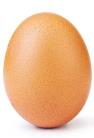
\includegraphics[height=1.75cm]{../img/ch6-egg-clean.png}};
  \node[inner sep=0] (broken) at (4.6,-0.1)
    {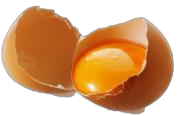
\includegraphics[height=1.48cm]{../img/ch6-egg-broken-clean.png}};
  \draw[flow] (0.75,0.35) .. controls (1.8,1.15) and (2.8,1.15) .. (3.45,0.45);
  \node[lbl, duBlue] at (2.1,1.25) {$S_\text{gen} > 0$};
  \draw[flow] (3.45,-0.55) .. controls (2.8,-1.25) and (1.8,-1.25) .. (0.75,-0.65);
  \cross{(2.1,-1.05)}
  % --- hot cup in a 20 C room --------------------------------------------
  \begin{scope}[shift={(8.6,0)}]
    \foreach \x/\t in {0/100, 4.2/20} {
      \draw[line width=1.26pt] (\x-1.0,-0.4) -- (\x+1.0,-0.4);          % table
      \draw[line width=1.26pt] (\x-0.6,-0.4) rectangle (\x+0.6,0.45);   % cup
      \node[lbl] at (\x,0.02) {$\t\,^\circ$C};
      \node[lbl] at (\x,0.8) {$20\,^\circ$C};
    }
    \draw[-{Stealth[length=2.6mm]}, line width=1.68pt] (0.9,0.05) -- (3.3,0.05);
    \draw[flow] (3.4,-0.6) .. controls (2.8,-1.2) and (1.4,-1.2) .. (0.8,-0.6);
    \cross{(2.1,-1.05)}
  \end{scope}
\end{tikzpicture}
\end{document}
